\section{Exercise 2}
\subsection*{2.1}
To prove $\tilde{I}_1(x,y)  = \tilde{I}_2(x,y) = \frac{a+b}{2}$ we first look into the CDF and the inverse CDF for the images. For a constant image, the CDF would be 0 until it reaches the constant and then it spikes to 1. If we compute $CDF(I(x,y))$ of a constant image we will get 1 for all the pixels because all the pixels have the same intensity. The inverse CDF  gives us the value corresponding to the probability. For a constant image, if we take $CDF(I(x,y))$ we get the probability 1, and if we then take $CDF^{-1}(1)$ we get the intensity of the constant image.\\
For this exercise we have $C_1$ and $C_2$. Taking $C_1(I_1(x,y))$ gives us 1 as $I_1$ is constant. Taking $C_1^{-1}(C_1(I_1(x,y)))$ thus simply gives us the pixel intensity of $I_1(x,y) = a$ back. But taking $C_2^{-1}(C_1(I_1(x,y)))$ gives us the constant value of $I_2$ back, as $C_2$ spikes at the constant value of $I_2$ which is $b$.\\
We thus have:
\begin{align*}
	\tilde{I}_1 &= \frac{1}{2}\left(C_1^{-1}(C_1(I_1)) + C_2^{-1}(C_1(I_1))\right)\\
	&= \frac{1}{2}\left(C_1^{-1}(1) + C_2^{-1}(1)\right)\\
	&= \frac{1}{2}\left(a + b\right)\\
\end{align*}
And:
\begin{align*}
	\tilde{I}_2 &= \frac{1}{2}\left(C_1^{-1}(C_2(I_2)) + C_2^{-1}(C_2(I_2))\right)\\
	&= \frac{1}{2}\left(C_1^{-1}(1) + C_2^{-1}(1)\right)\\
	&= \frac{1}{2}\left(a + b\right)\\
\end{align*}
And we have thus proved $\tilde{I}_1(x,y)  = \tilde{I}_2(x,y) = \frac{a+b}{2}$.\\
As $\frac{a+b}{2}$ gives us the average value, the resulting CDF will spike at the average, and thus the cumulative histogram of the midway specification is equal to the average of the cumulative histograms.

\subsection*{2.2}
\begin{figure}[H]
	\centering
	\begin{subfigure}[b]{0.45\textwidth}
		\centering
		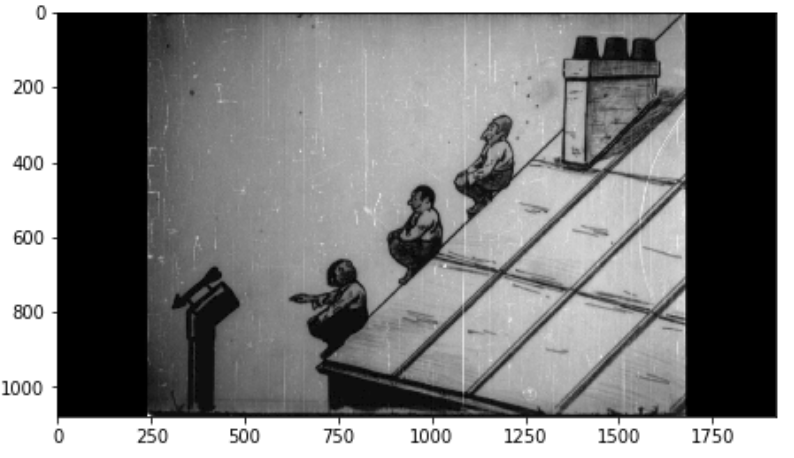
\includegraphics[width=\textwidth]{Materials/ms1}
		\caption{Midway specification of 'movie\_flicker1' image.}
	\end{subfigure}
	\hfill
	\begin{subfigure}[b]{0.45\textwidth}
		\centering
		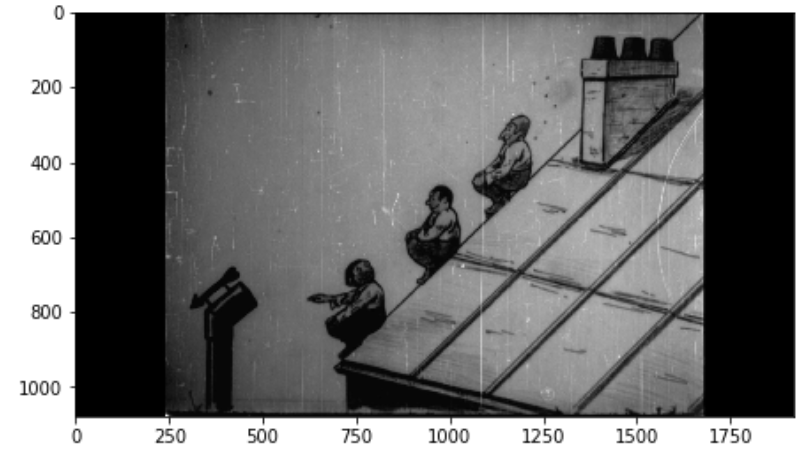
\includegraphics[width=\textwidth]{Materials/Flicker1}
		\caption{Original 'movie\_flicker1'.}
	\end{subfigure}
	\hfill
	\\
	\begin{subfigure}[b]{0.45\textwidth}
		\centering
		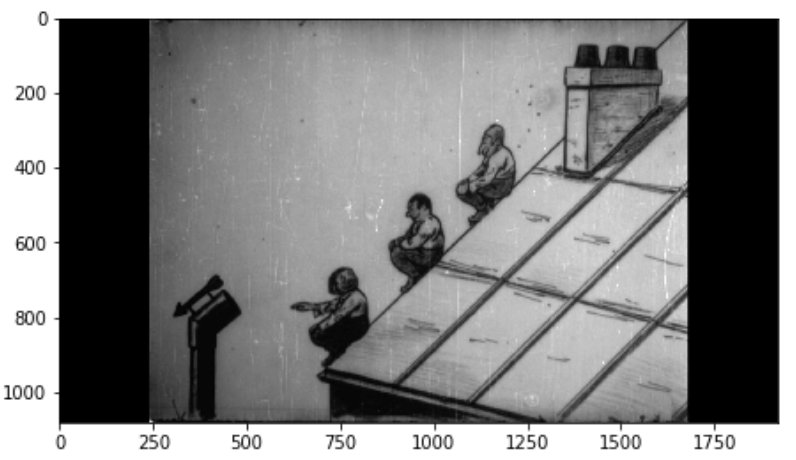
\includegraphics[width=\textwidth]{Materials/ms2}
		\caption{Midway specification of 'movie\_flicker2' image.}
	\end{subfigure}
	\hfill
	\begin{subfigure}[b]{0.45\textwidth}
		\centering
		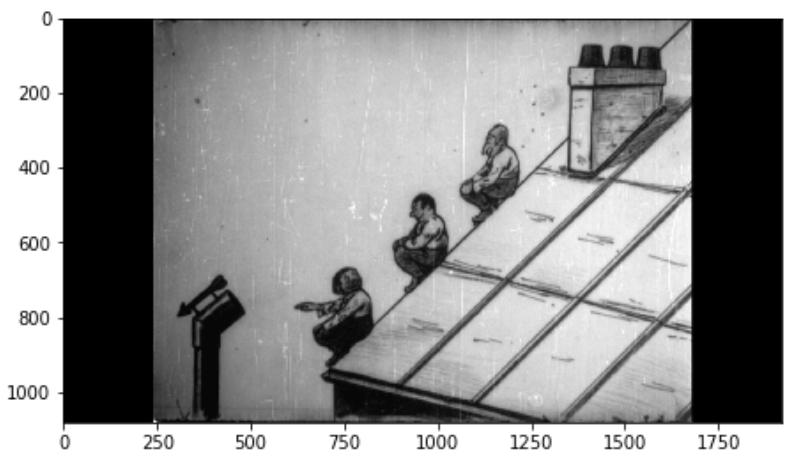
\includegraphics[width=\textwidth]{Materials/Flicker2}
		\caption{Original 'movie\_flicker2'.}
	\end{subfigure}
	\caption{Midway specification and original images.}
	\label{midway}
\end{figure}

\begin{figure}[H]
	\centering
	\begin{subfigure}[b]{0.45\textwidth}
		\centering
		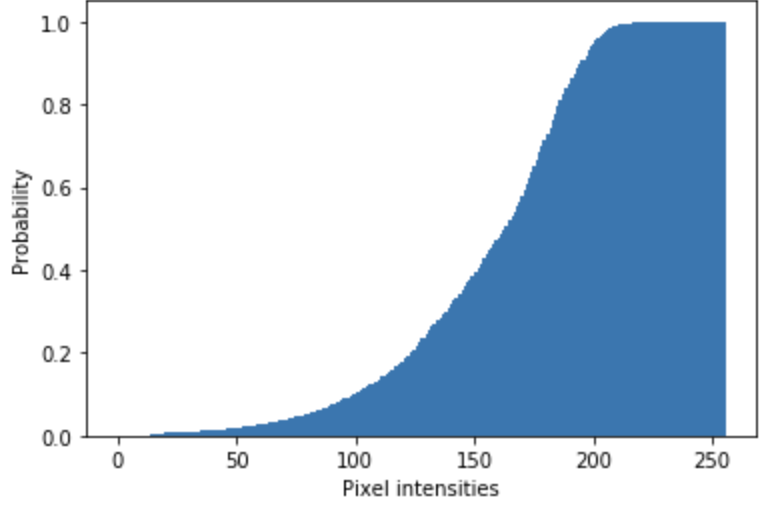
\includegraphics[width=\textwidth]{Materials/cdfms1}
		\caption{CDF of Midway specification of 'movie\_flicker1' image.}
	\end{subfigure}
	\hfill
	\begin{subfigure}[b]{0.45\textwidth}
		\centering
		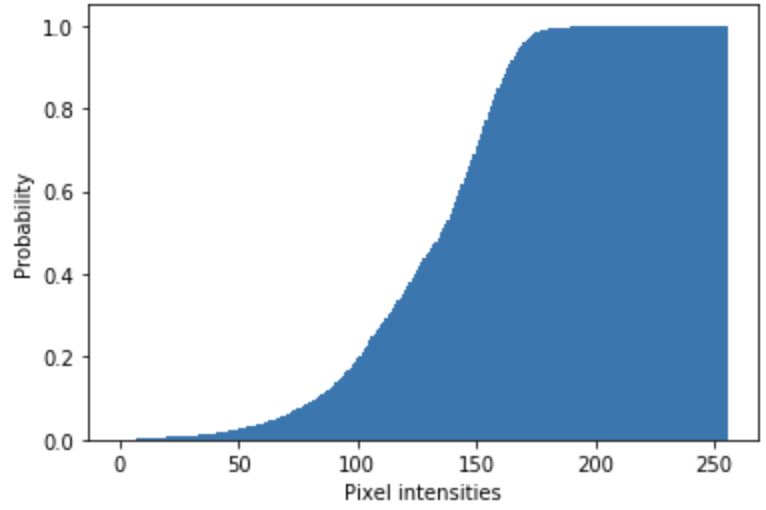
\includegraphics[width=\textwidth]{Materials/cdfmf1}
		\caption{CDF of Original 'movie\_flicker1'.\\\hfill}
	\end{subfigure}
	\hfill
	\\
	\begin{subfigure}[b]{0.45\textwidth}
		\centering
		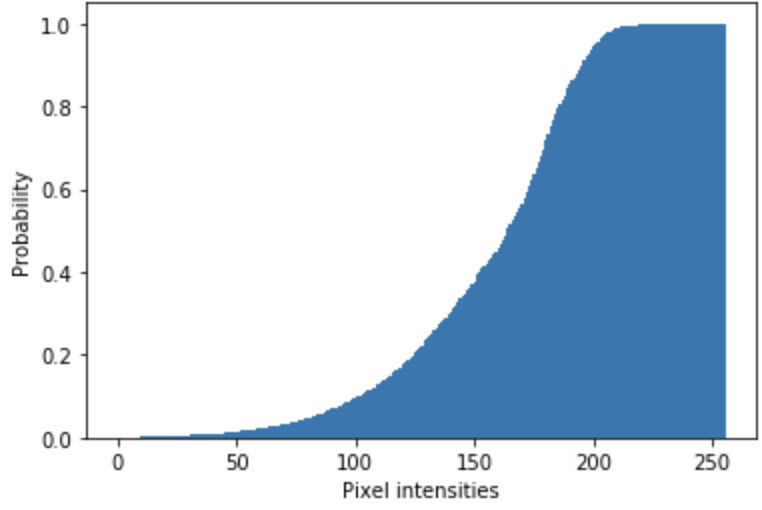
\includegraphics[width=\textwidth]{Materials/cdfms2}
		\caption{CDF of Midway specification of 'movie\_flicker2' image.}
	\end{subfigure}
	\hfill
	\begin{subfigure}[b]{0.45\textwidth}
		\centering
		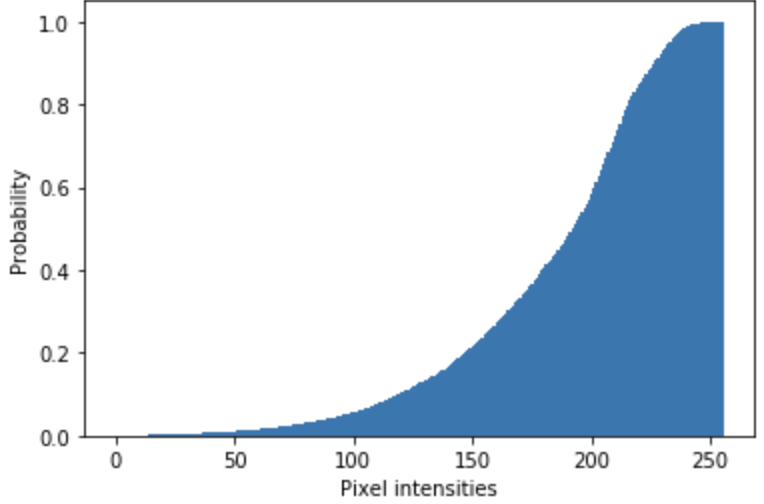
\includegraphics[width=\textwidth]{Materials/cdfmf2}
		\caption{Original 'movie\_flicker2'.\\\hfill}
	\end{subfigure}
	\caption{CDF of Midway specification and original images.}
	\label{cdf}
\end{figure}
In \autoref{midway} we see the midway specifications of the two images \textit{'movie\_flicker1'} and \textit{'movie\_flicker2'} together with the original images. In \autoref{cdf} we see their CDFs. To generalize the midway specification function $\phi$ we would define it as:
\begin{equation*}
	\phi(x) = \frac{1}{N}\left(C_1^{-1}(x)+C_2^{-1}(x)+...+C_N^{-1}(x)\right)
\end{equation*}
Where $N$ is the number of images. We would then get the \textit{n}'th midway specification as $\tilde{I}_n = \phi(C_n(I_n))$.\\
The code for this exercise can be seen in \autoref{e2code}. The 'cdf' function returns a list of probabilities (one for each pixel intensity) and the corresponding pixel intensities. The utility functions not shown have been reused from last week's assignment.
\begin{figure}[H]
	\centering
	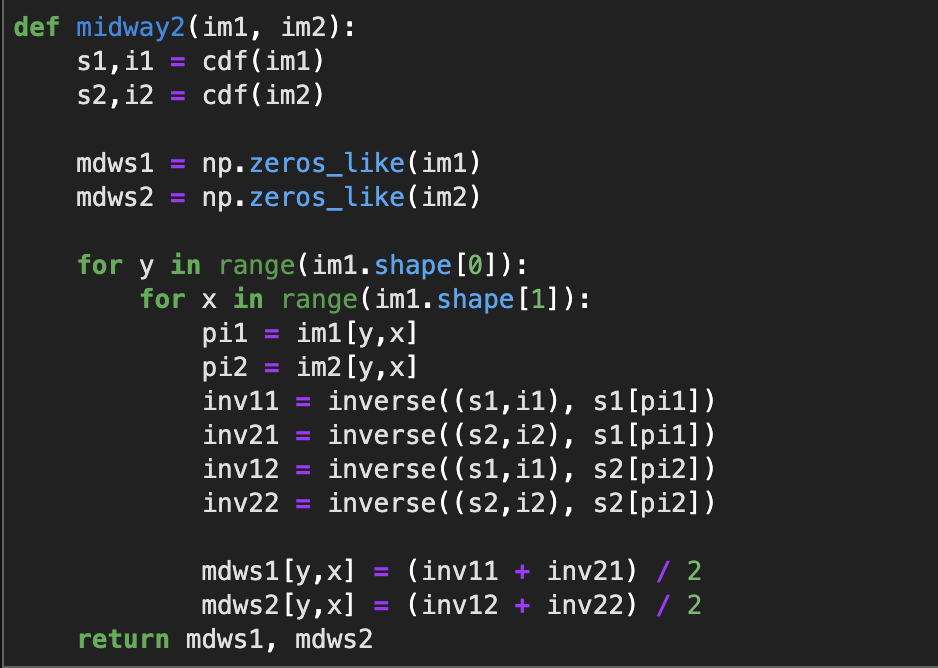
\includegraphics[width=0.7\linewidth]{Materials/e2code}
	\caption{Code for exercise 2.}
	\label{e2code}
\end{figure}